%--------------------------------------------------------------------------------------------------
\section{Preliminaries} \label{sec:Preliminaries} 
%--------------------------------------------------------------------------------------------------

Deliverable 3.1 introduced a thorough and up-to-date description of the state-of-the art of inference in hybrid and dynamic Bayesian networks \cite{Deliverable 3.1}.

Intorduction to Variational Inference \cite{Jordan1999,Attias2000}, conjugate-exponential families \cite{Attias2000,Beal2003,Bishop2005}

An overview of the data structures implemented in the AMIDST toolbox is illustrated in Figure \ref{Figure:ToolboxDataStructures}. These data structures, described in Deliverable 2.3 \cite{Deliverable2.3}, define the core components used by the AMIDST inference algorithms. 


\begin{figure}[ht!]
\begin{center}
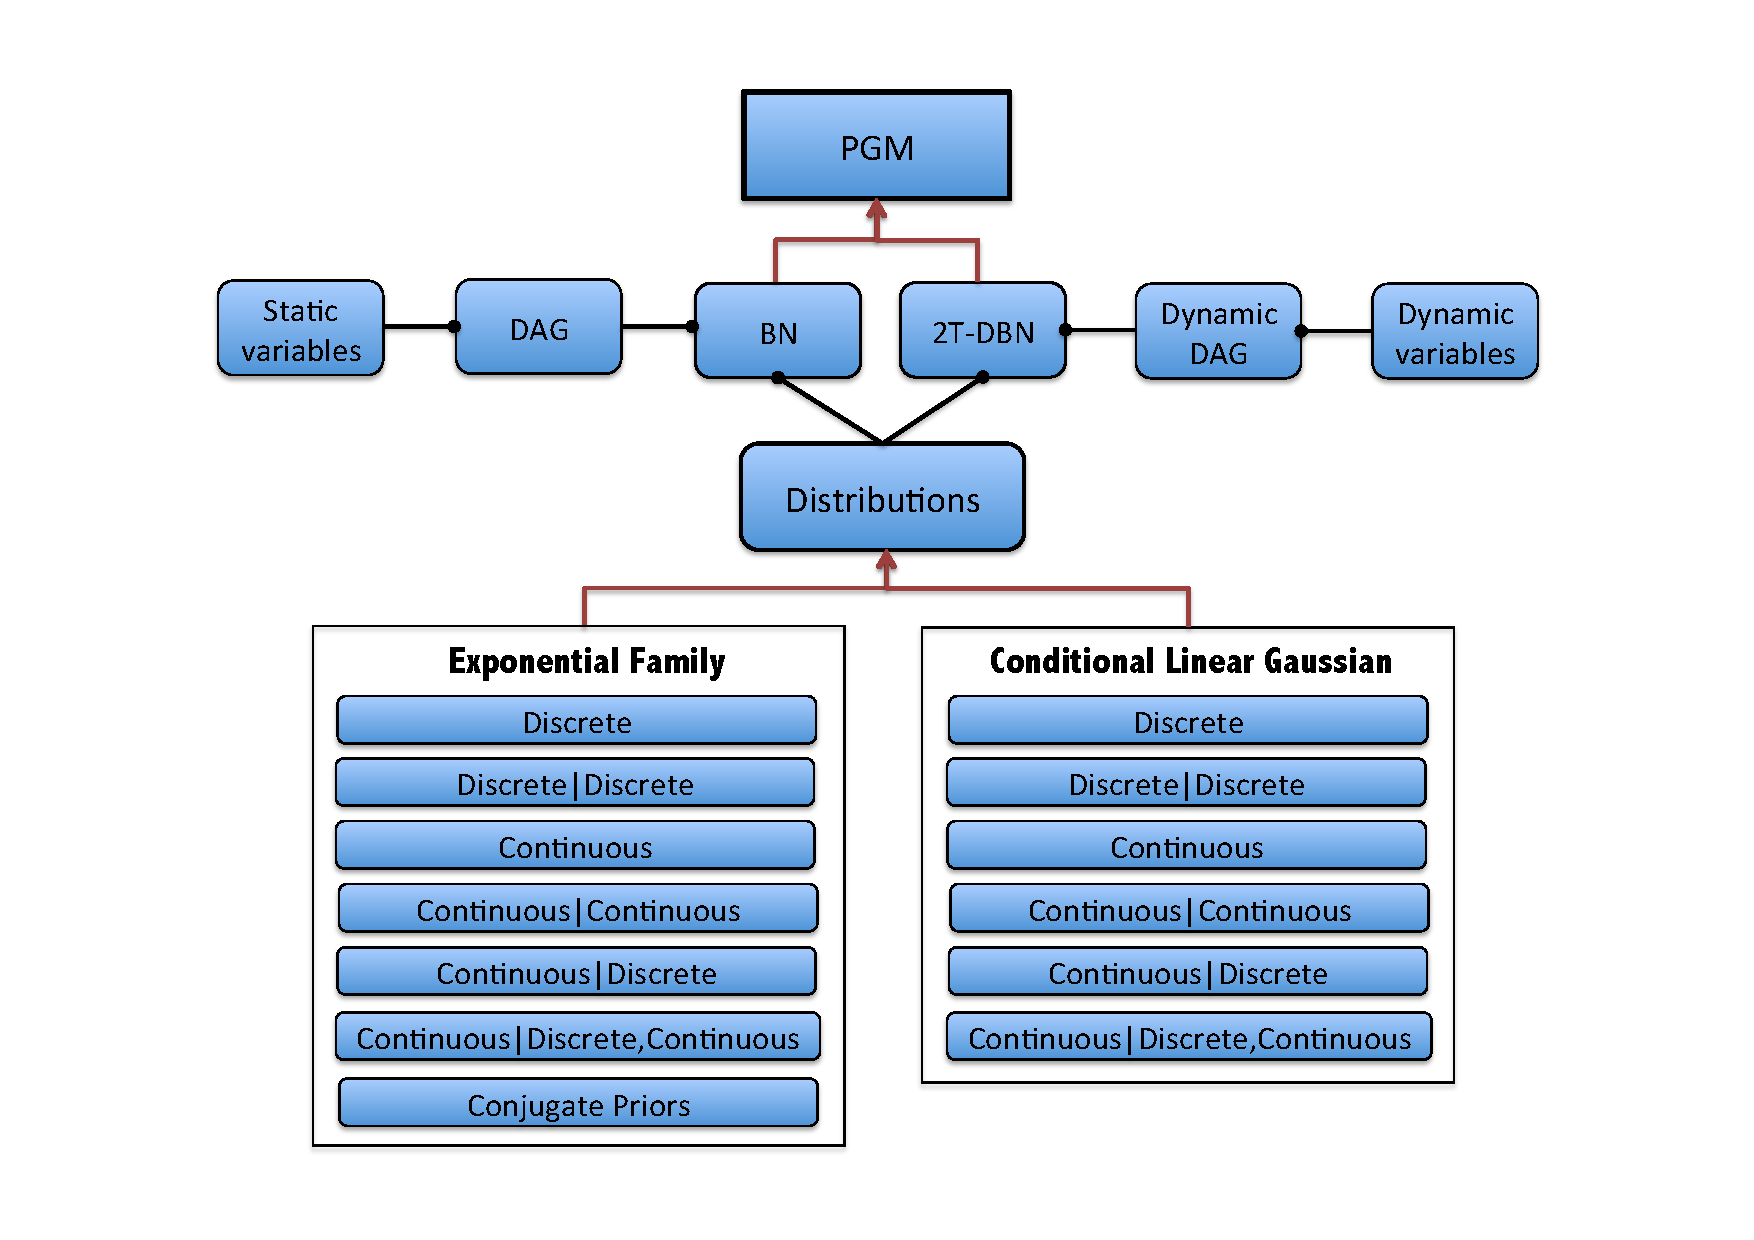
\includegraphics[width=\linewidth]{./figures/DataStructure}
\vspace{-0.5in}
\caption{\label{Figure:ToolboxDataStructures} Illustration of AMIDST toolbox data structure components. Nomenclature: The boxes in the
      figure represent software components (sets, possibly singletons, of classes), a rounded-arc going from $X$ to $Y$ indicates that $Y$ 'uses/references' $X$, and an arc with an arrow from $X$ to $Y$ implies inheritance.}
\end{center}
\end{figure}